% ++++++++++++++++++++++++++++++++++++++++
% Don't modify this section unless you know what you're doing!
\documentclass[a4paper,12pt]{article}
\usepackage{tabularx} % extra features for tabular environment
\usepackage{amsmath}  % improve math presentation
\usepackage{graphicx} % takes care of graphic including machinery
\usepackage[margin=0.75in]{geometry} % decreases margins
\usepackage{subcaption}
\usepackage{verbatim}
\usepackage{float}
\usepackage{hyperref}
\usepackage{titling}
\hypersetup{
	colorlinks=true,       % false: boxed links; true: colored links
	linkcolor=black,        % color of internal links
	citecolor=blue,        % color of links to bibliography
	filecolor=magenta,     % color of file links
	urlcolor=blue         
}
%++++++++++++++++++++++++++++++++++++++++
\setlength{\parindent}{0pt}
\setlength\parskip{0.5em plus 0.1em minus 0.2em}
\setlength{\droptitle}{-5em}   % This is your set screw

\begin{document}
\title{DC And AC Currents Through LCR Circuits \\
\large PHY224 Fall 2021}
\author{Fredrik Dahl Bråten, Pankaj Patil}
\date{\today}
\maketitle
\begin{center}
	\section*{Abstract}
\end{center}
The aim of this experiment is  to study the behavior of different circuit elements, like 
Resistors, Capacitors and Inductors in DC and AC circuits. We observed that a capacitor opposes
increase in charge accumulation, while an Inductor opposes changes in the current passing through it. As a result, a Capacitor in a DC circuit is an open
circuit, while an Inductor in a DC circuit is a short circuit. In this report we present 
these behaviors with the help of Oscilloscope measurements.

\section{Introduction}

\subsection*{A. Background Theory}
In a RC circuit, the voltage of the capacitor is given by $V_0 = \frac{Q_0}{C} \ \text{, and as we know  } I_0 = \frac{V_R}{R} \implies V_R = V_0e^{-\frac{t}{\tau}}\ \text{, where } \tau = RC$. This is also 
the fitting equation for this case. Here the measured time is our independent variable, while $V_R$ across the resistor is our dependent variable. The capacitance (C) and the the resistance (R) are 
auxiliary parameters.

In a LR circuit, we have $I_R(t) = I_0(1-e^{\frac{t}{L/R}}) \implies V_R =  V_0(1-e^{\frac{t}{L/R}})$, where $I_0  = \frac{V_0}{R}$. Our fitting equation is the same, and again time is our 
independent variable, and voltage across the Resistor $V_R$, is the dependent variable. $L$ and $R$ are auxiliary parameters.

In a LCR circuit, the total impedance $Z$ is defined as $Z = \sqrt{(\omega L - \frac{1}{\omega C})^2 + R^2}$. $Z$ can be found by measuring 
the total Voltage $V$, compared to the voltage $V_R = RI \implies Z = \frac{V}{V_R}R$.

It is clear from the fitting equation for the RC circuit that we would observe exponential decay for the Voltage across the resistor, as can be seen in Figure \ref{Combined_RC_B}. In the case of the LR circuit, the relationship is reversed, and we observe exponential increase 
in voltage across the Resistor, as seen in Figure \ref{Combined_LR_W}.

\subsection*{B. Materials and Methods}

In this experiment we used various circuit elements namely Resistors, Capacitors, and Inductors, in the setups provided
in the lab manual \cite{lab-manual-ex7}. The measurements were made by connecting the two wires of the channels of the Oscilloscope to each side of the circuit element(s) for which we wanted to measure voltage across over time.

We followed the steps provided in the lab manual \cite{lab-manual-ex7} for this 
experiment. We also made adjustments based on TA's suggestion to the circuits as the 
AC circuits in the manual were applicable to old Oscilloscopes.

\section{Results}
\subsection*{A. Transient Decay (RC)}

\begin{figure}[H]
  \centerline{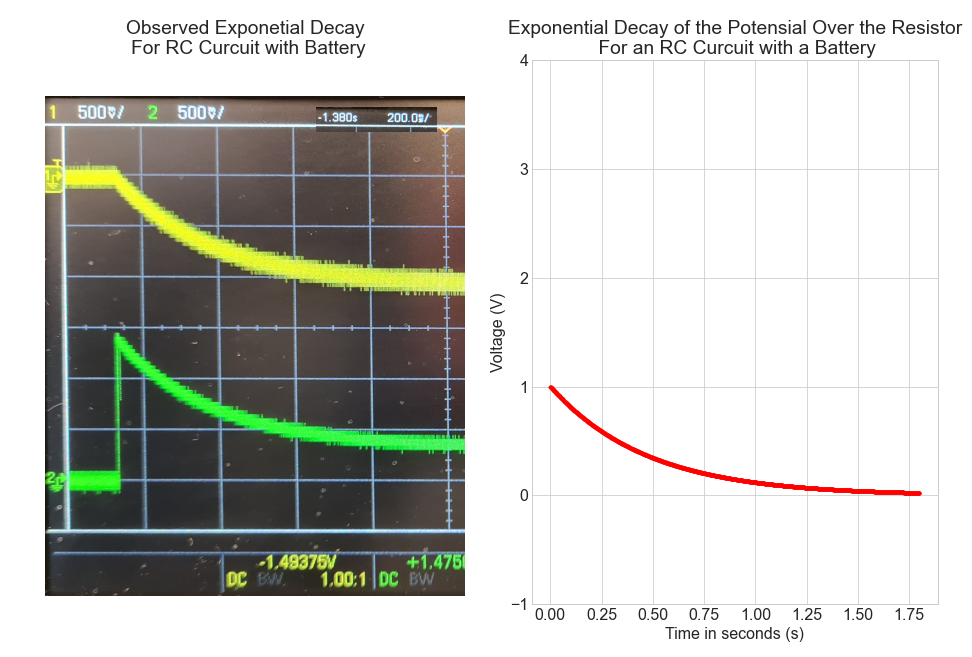
\includegraphics[width=0.5\textwidth]{../Simulated Curves/RC_B-mod.png}}
  \caption{Transient Potential Decay in RC circuit (Measurement Vs. Simulation)}
  \label{Combined_RC_B}
\end{figure}
$$\tau\ (measured) = 0.4\ s, \ \ RC = 0.47\ s$$

The estimated value of the time constant, estimated from our measurements, matches the theoretical value $RC$ closely. 

\subsection*{B. DC Square Wave}

\begin{figure}[H]
  \centerline{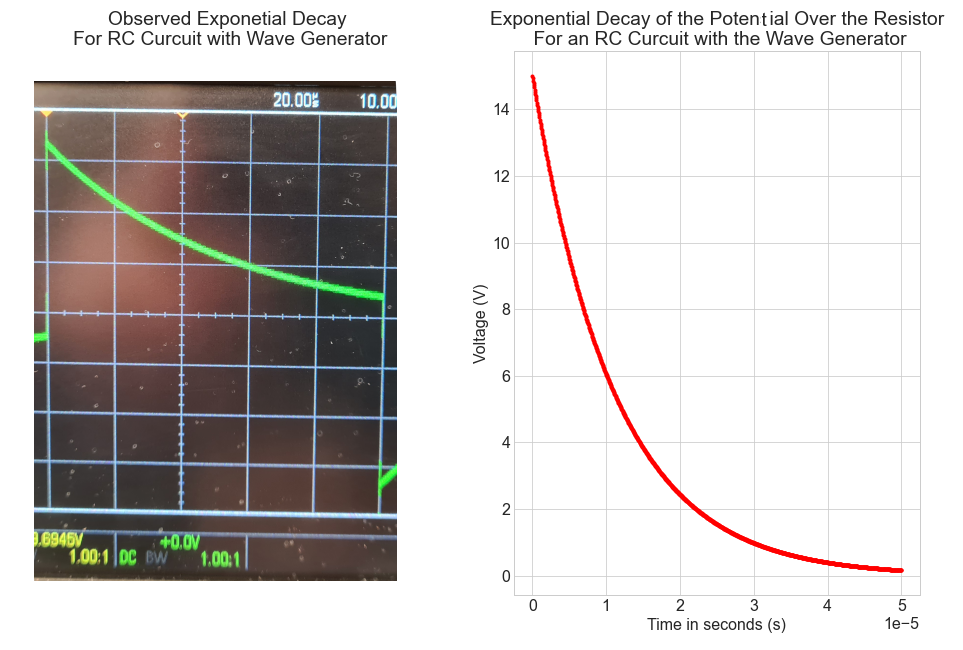
\includegraphics[width=0.5\textwidth]{../Simulated Curves/RC_W-mod.png}}
  \caption{Exponential Potential Decay in RC circuit (Measurement Vs. Simulation)}
  \label{Combined_RC_W}
\end{figure}
$$\tau\ (measured) = 8 \times 10^{-5}\ s$$
$$RC = 1.1 \times 10^{-5}\ s$$

The estimated value of the time constant, estimated from our measurements, matches the theoretical value $RC$ in order of magnitude. 

\begin{figure}[H]
  \centerline{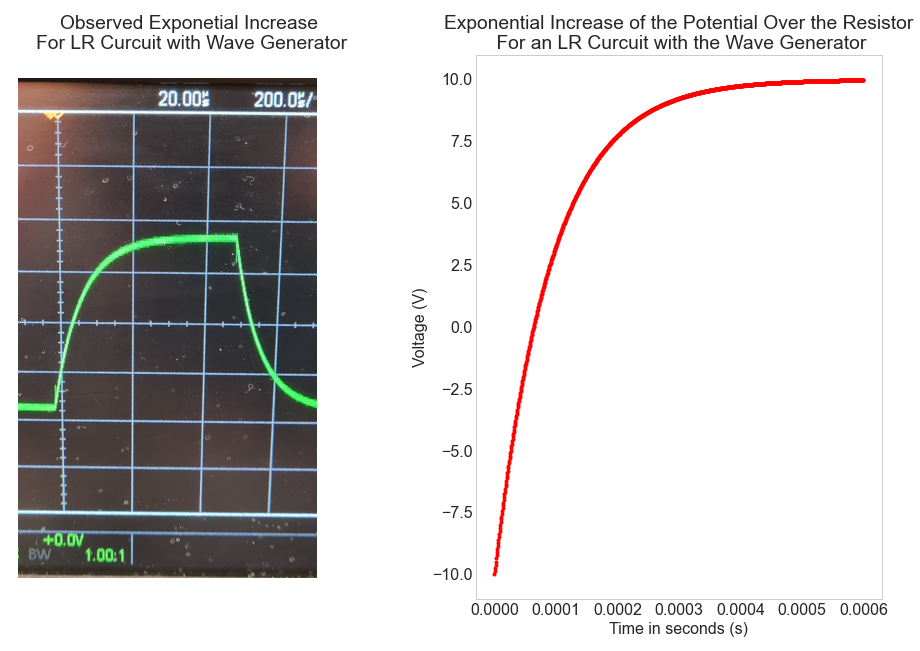
\includegraphics[width=0.75\linewidth]{../Simulated Curves/LR_W-mod.png}}
  \caption{Exponential Potential Increase in LR circuit (Measurement Vs. Simulation)}
  \label{Combined_LR_W}
\end{figure}
$$\tau\ (measured) = 5.0 \times 10^{-5}\ s$$
$$L/R = 9.2 \times 10^{-5}\ s$$

The estimated value of the time constant, estimated from our measurements, matches the theoretical value $L/R$ in order of magnitude. 
All these three theoretical curves matches our measured curves well, and as mentioned, gives time constants within an order of magnitude of the measured values.
\\\\
\begin{figure}[H]
  \centering
  \begin{subfigure}{.5\textwidth}
    \centering
    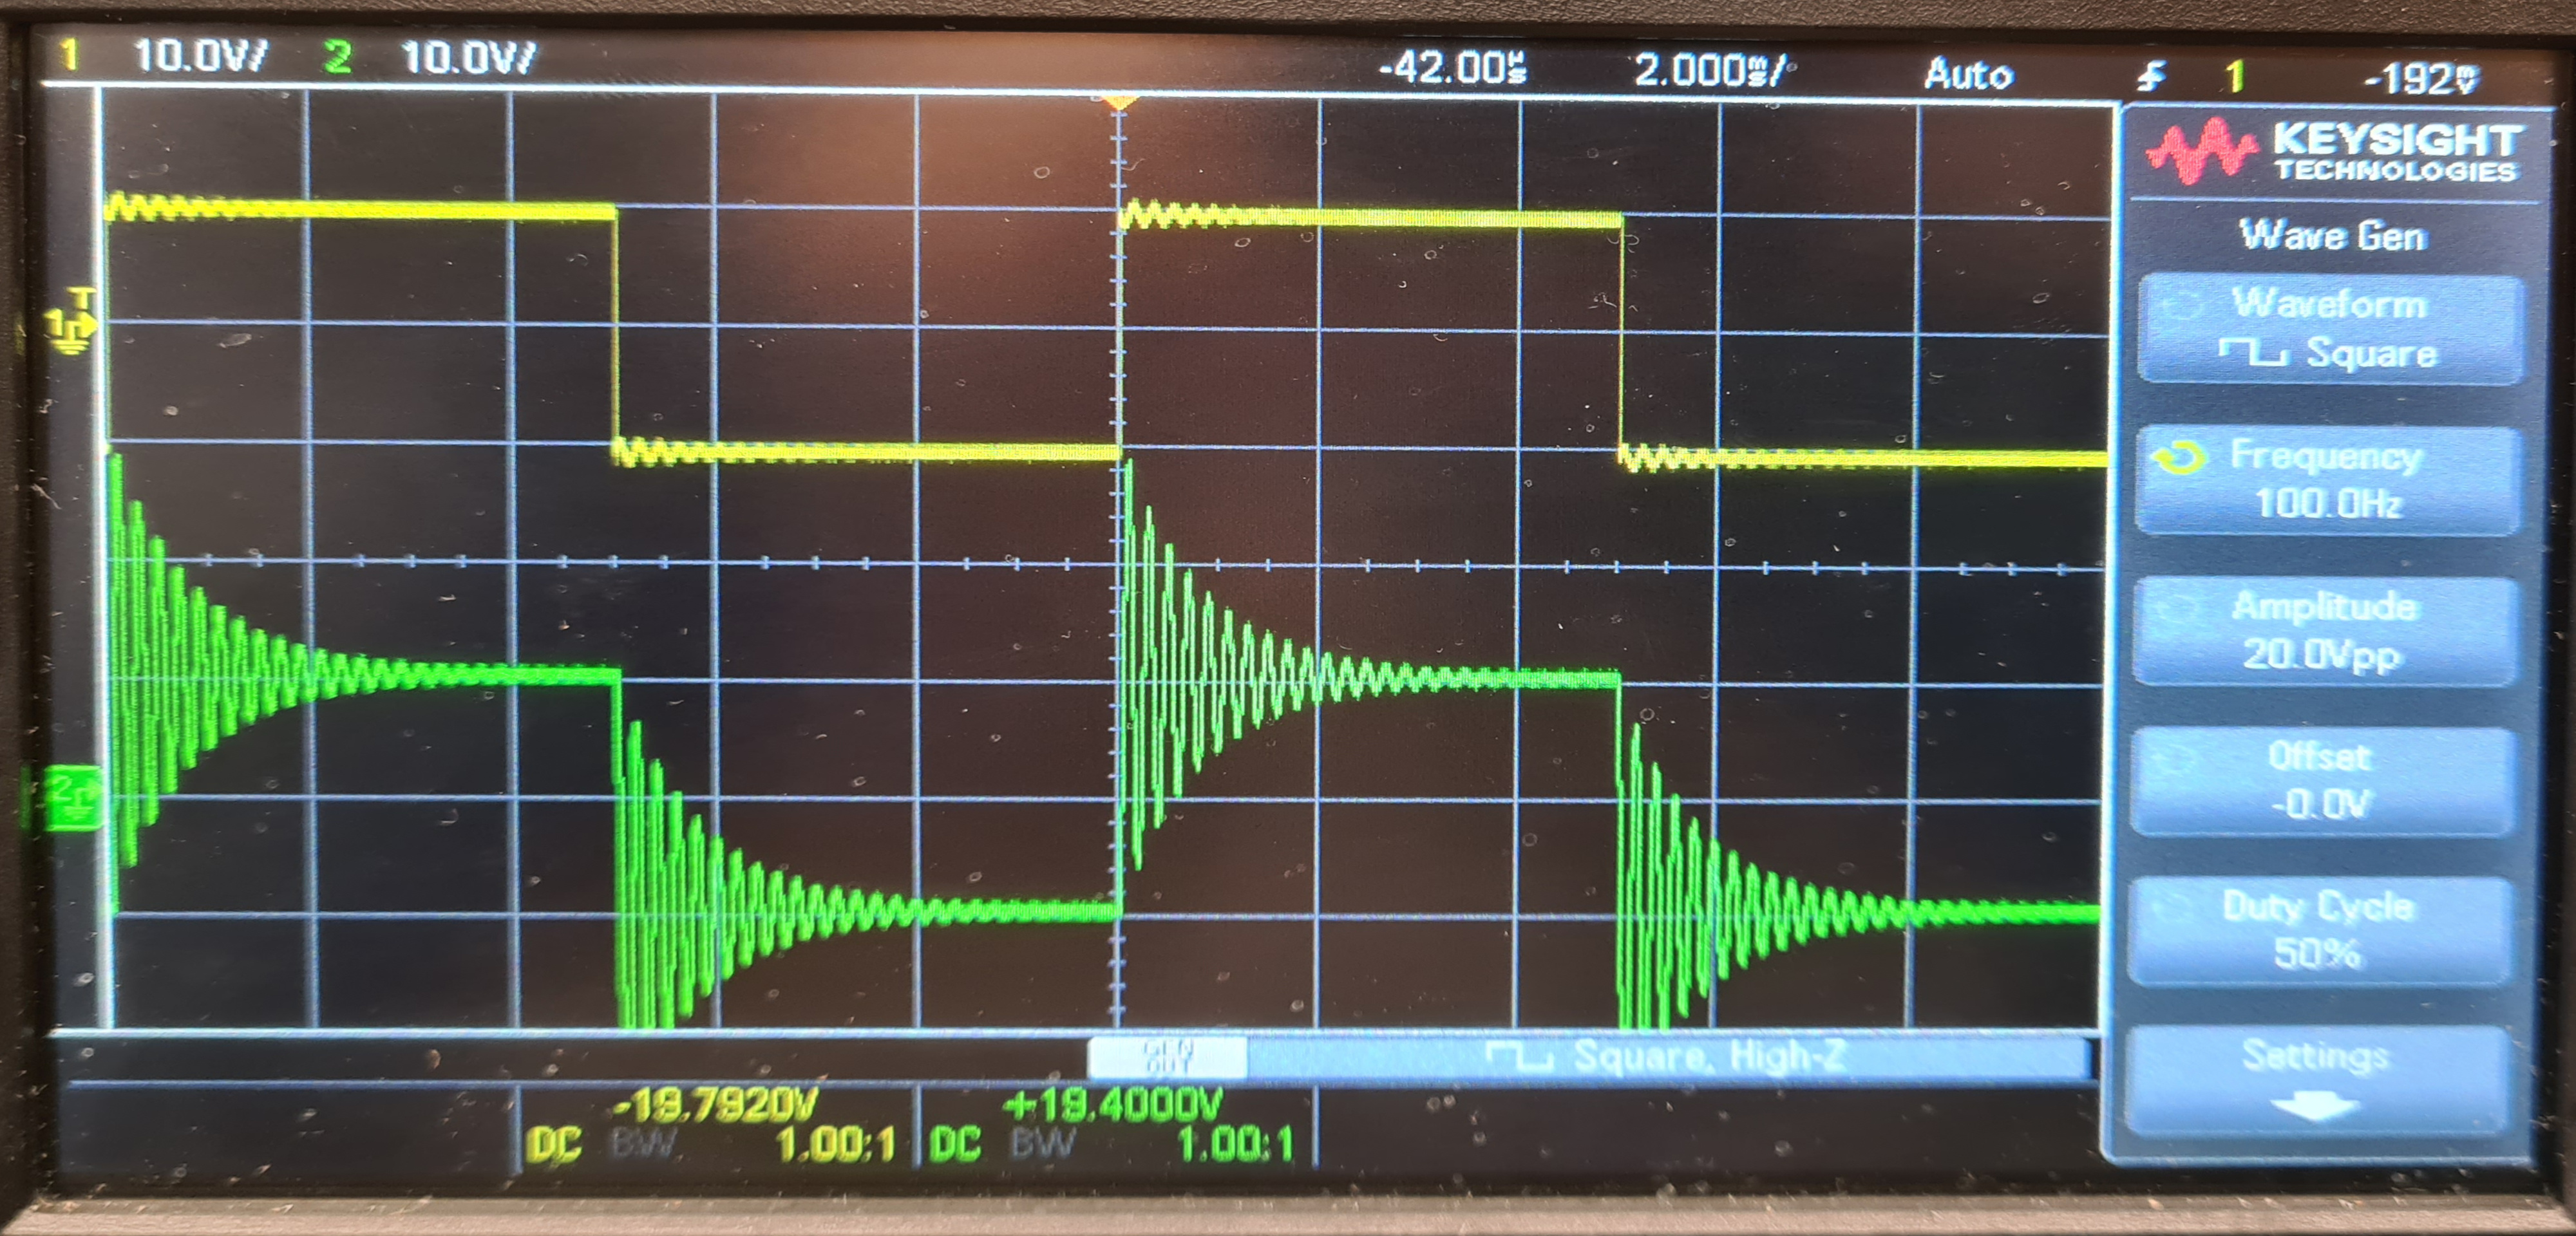
\includegraphics[width=.9\linewidth]{../data/20211116_110612-mod.jpg}
    \caption{LC Circuit with Square Wave}
  \end{subfigure}%
  \begin{subfigure}{.5\textwidth}
    \centering
    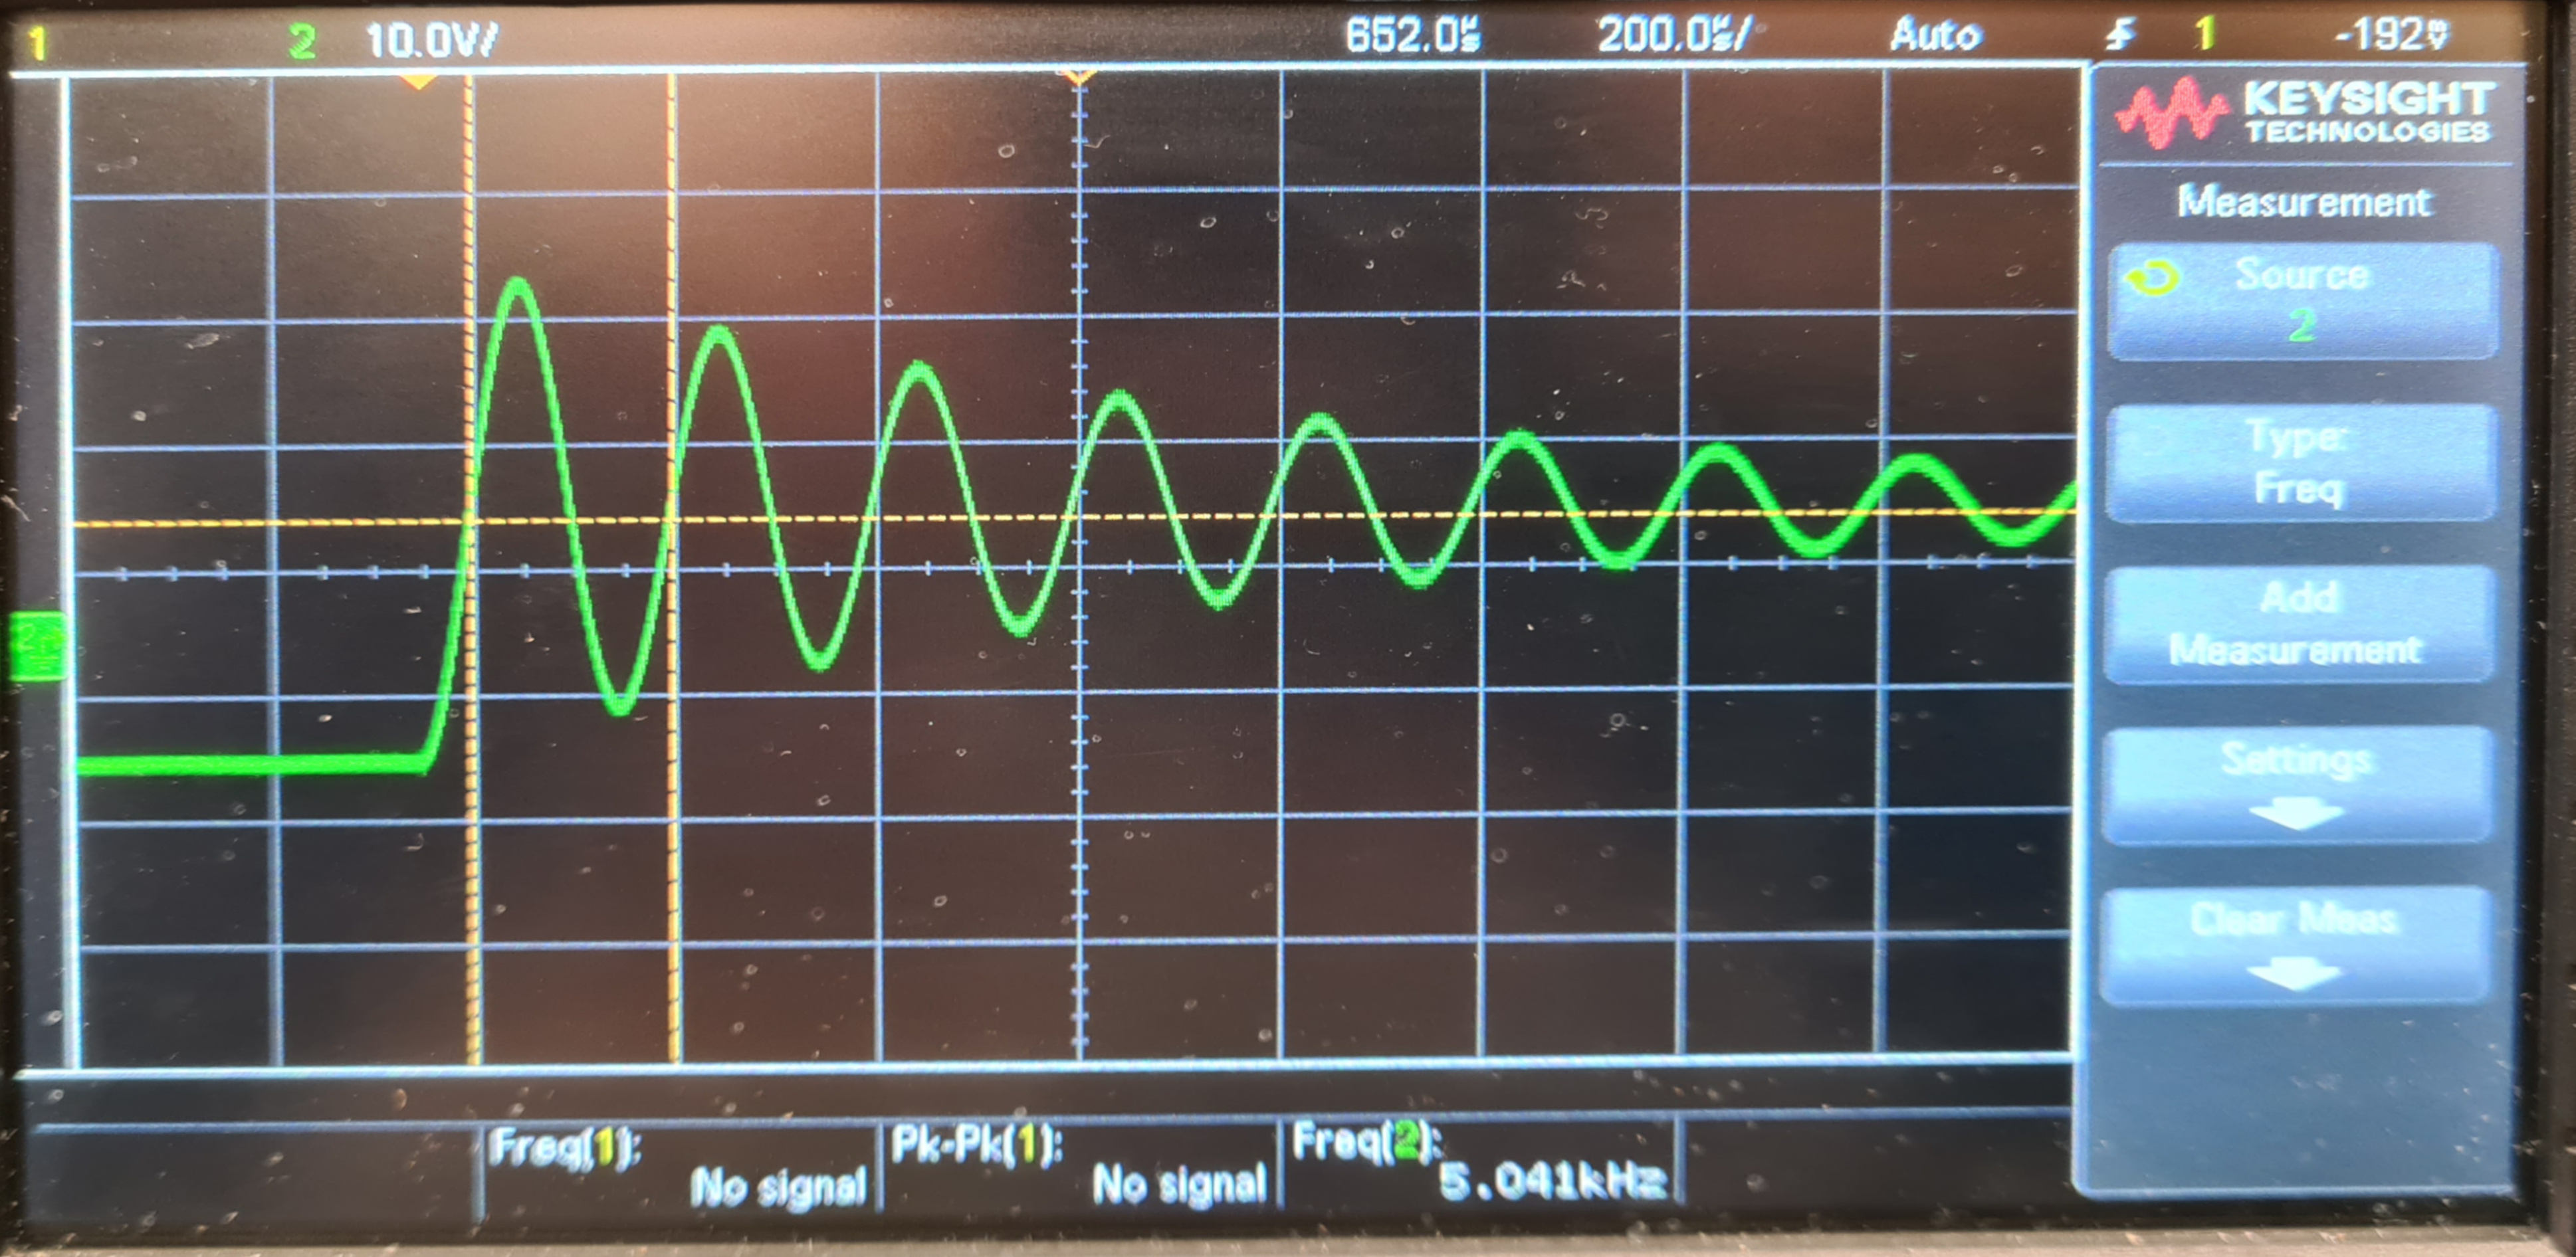
\includegraphics[width=.9\linewidth]{../data/20211116_110834-mod.jpg}
    \caption{LC Circuit with Square Wave (Zoomed In)}
  \end{subfigure}
  \caption{LC Circuit}
\end{figure}

For the LC circuit, the observed behavior is different from the theoretically predicted one. This is because we 
can never make pure LC circuit, as there will always be some resistance in the circuit which will cause damping.

\subsection*{C. AC Sine Wave}

\begin{figure}[H]
  \centering
  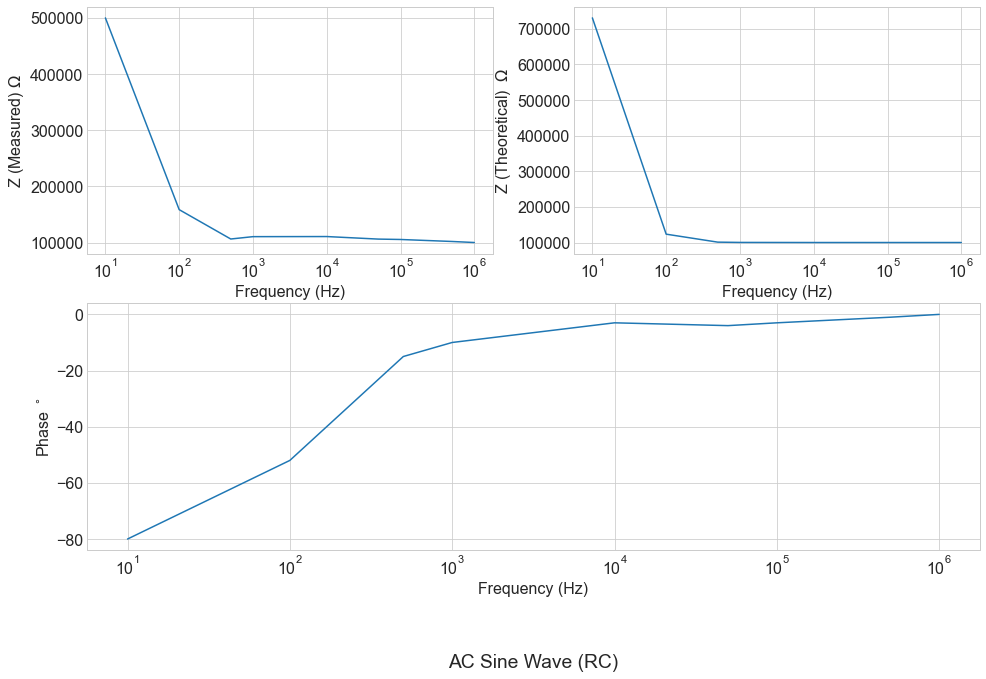
\includegraphics[width=0.8\linewidth]{../code/AC Sine Wave (RC).png}    
  \caption{AC Sine Wave (RC): Z vs Frequency and Phase vs Frequency Plots}
  \label{Combined_RC_AC}
\end{figure}

\begin{figure}[H]
  \centering
  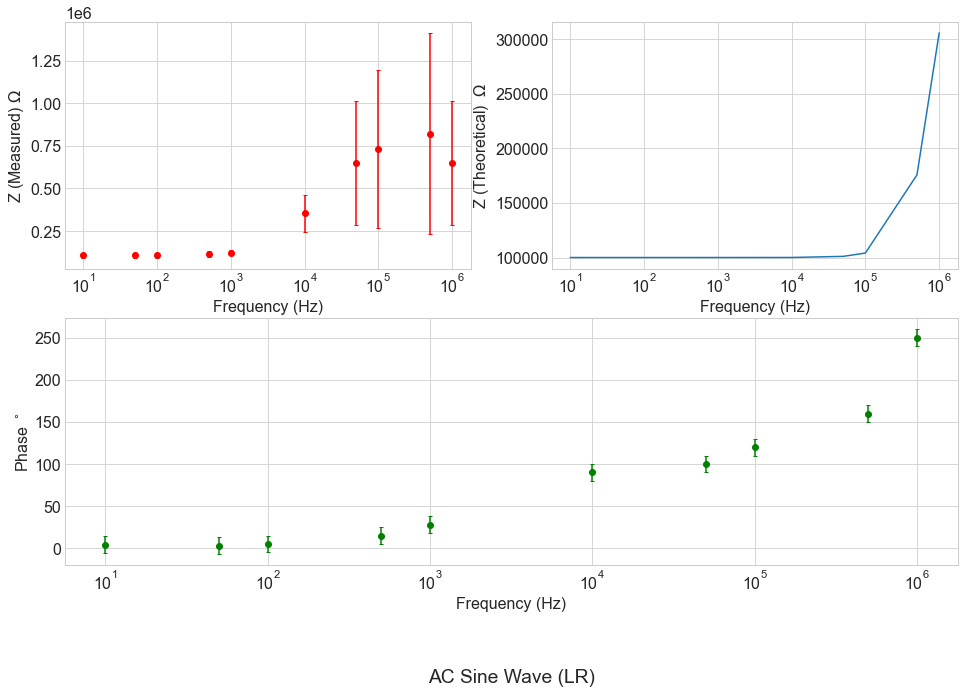
\includegraphics[width=0.8\linewidth]{../code/AC Sine Wave (LR).png}    
    \caption{AC Sine Wave (LR): Z vs Frequency and Phase vs Frequency Plots}
    \label{Combined_LR_AC}
\end{figure}

\begin{figure}[H]
  \centering
  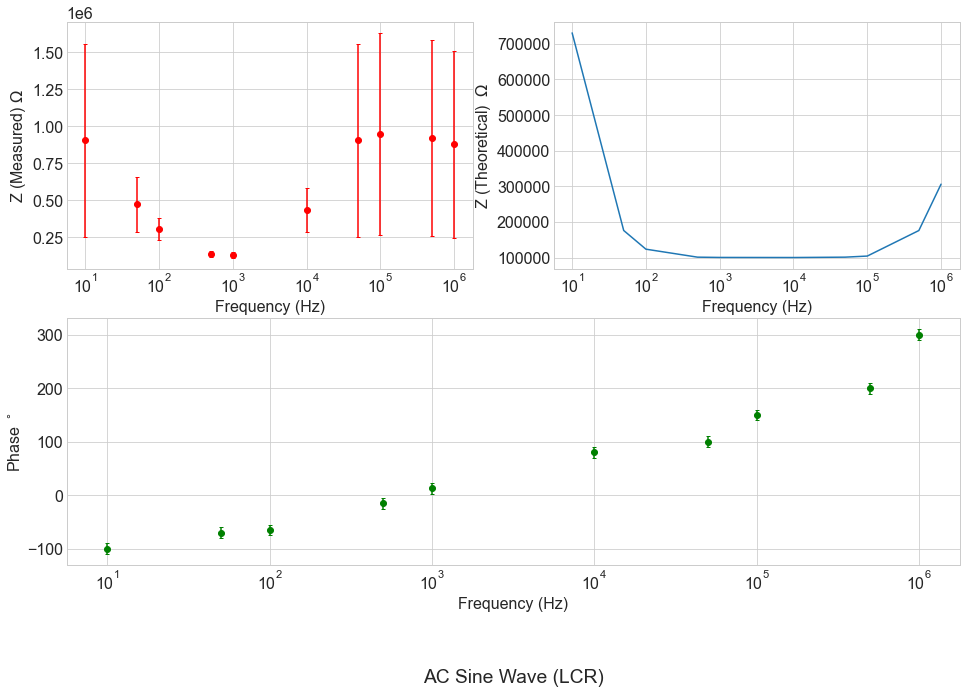
\includegraphics[width=0.8\linewidth]{../code/AC Sine Wave (LCR).png}    
    \caption{AC Sine Wave (LCR): Z vs Frequency and Phase vs Frequency Plots}
    \label{Combined_LCR_AC}
\end{figure}

\section{Uncertainty}

For the purpose of this experiment, we estimated the uncertainty in $V_R$
as the thickness of the voltage line plotted on the Oscilloscope for channel 2. This channel 
measures the voltage across the Resistor. In case of the DC circuit, with the RC configuration, we observe that 
$\Delta V_R = \frac{1}{4} \times \text{Voltage Division} = .25 \times 500\ mV = 125\ mV$. 
And for the DC Square Wave, it is $2\ V$. Similarly for the LR Square Wave case, $\Delta V_R = 1\ V$.
Overall, for the experiment we can assume the uncertainty in the measurement of $V_R$ to be 
in order of magnitude 1 $V$.

\section{Discussion}

In the RC circuit, the accuracy of the measurement of $V_R$ in the DC case, is given by $\frac{|1.4/e - 1.|}{1.4/e} \times 100 = 35 \%$. 
And the precision of measurement of $V_R$ is given by $\frac{0.125}{0.7} \times 100 = 17 \%$. 
The accuracy value being large can be attributed to instrument error/inaccuracy.

In the LR circuit, the accuracy of $V_R$ in the DC case is given by $\frac{|12.64 - 10.0|}{12.64} \times 100 = 20 \%$. 
And the precision of measurement of $V_R$ is given by $\frac{1}{10} \times 100 = 10 \%$. 

In the LCR circuit for lower frequencies, the phase difference is negative. As the frequency is
increased, the phase gradually shifts to positive values. The resonance frequency can be estimated to be around 1 kHz. 
Furthermore, in accordance with theory, $\omega_r = 1/\sqrt{LC} = 1.4$ kHz.

From our LC circuit, we saw that we still had some resistance within the circuit. This is because an LC circuit would 
be an idealization of the actual LCR circuit for which we were really testing. Though the resistance was small, there was
some internal resistance within the capacitor and the inductor in our circuit, along with some internal resistance within the Oscilloscope.
Thus, we never managed to get data from a pure LC circuit. If one were to make a circuit diagram of our "LC" setup, using only ideal resistors, 
ideal capacitors, ideal inductors and an ideal oscilloscope, one would have to draw the LC circuit diagram for which can be found in the manual,
along with a small resistor in series right behind or right before the capacitor, the inductor and the oscilloscope, to account for their internal resistance.
In fact, the inductor does actually have some small capacitance as well, from accumulated charge between each wiring. Thus, a small capacitor 
would need to be drawn in the circuit diagram in series with the inductor as well, to capture the full picture of our imperfect LC circuit.

Given the capacitance, the inductance and the resistance within our LCR circuit, one can calculate the circuits natural resonance frequency.
Though driving the circuit with our wave generator at this natural frequency would give the largest resonance, one can also drive the circuit at all 
natural number multiples of this natural frequency and get some resonance. These are the overtones of the fundamental note, the natural frequency. 
This is similar to how one with musical instruments can achieve resonance on a string or in the air within a flute by playing the natural frequency or any 
of the overtones associated to the natural frequency of a string on a violin, a guitar, or associated to the pipes of a flute or an organ.


\pagebreak

\appendix

\section{Appendix}

\subsection{Oscilloscope Readings}

\begin{figure}[H]
  \centering
  \begin{subfigure}{.5\textwidth}
    \centering
    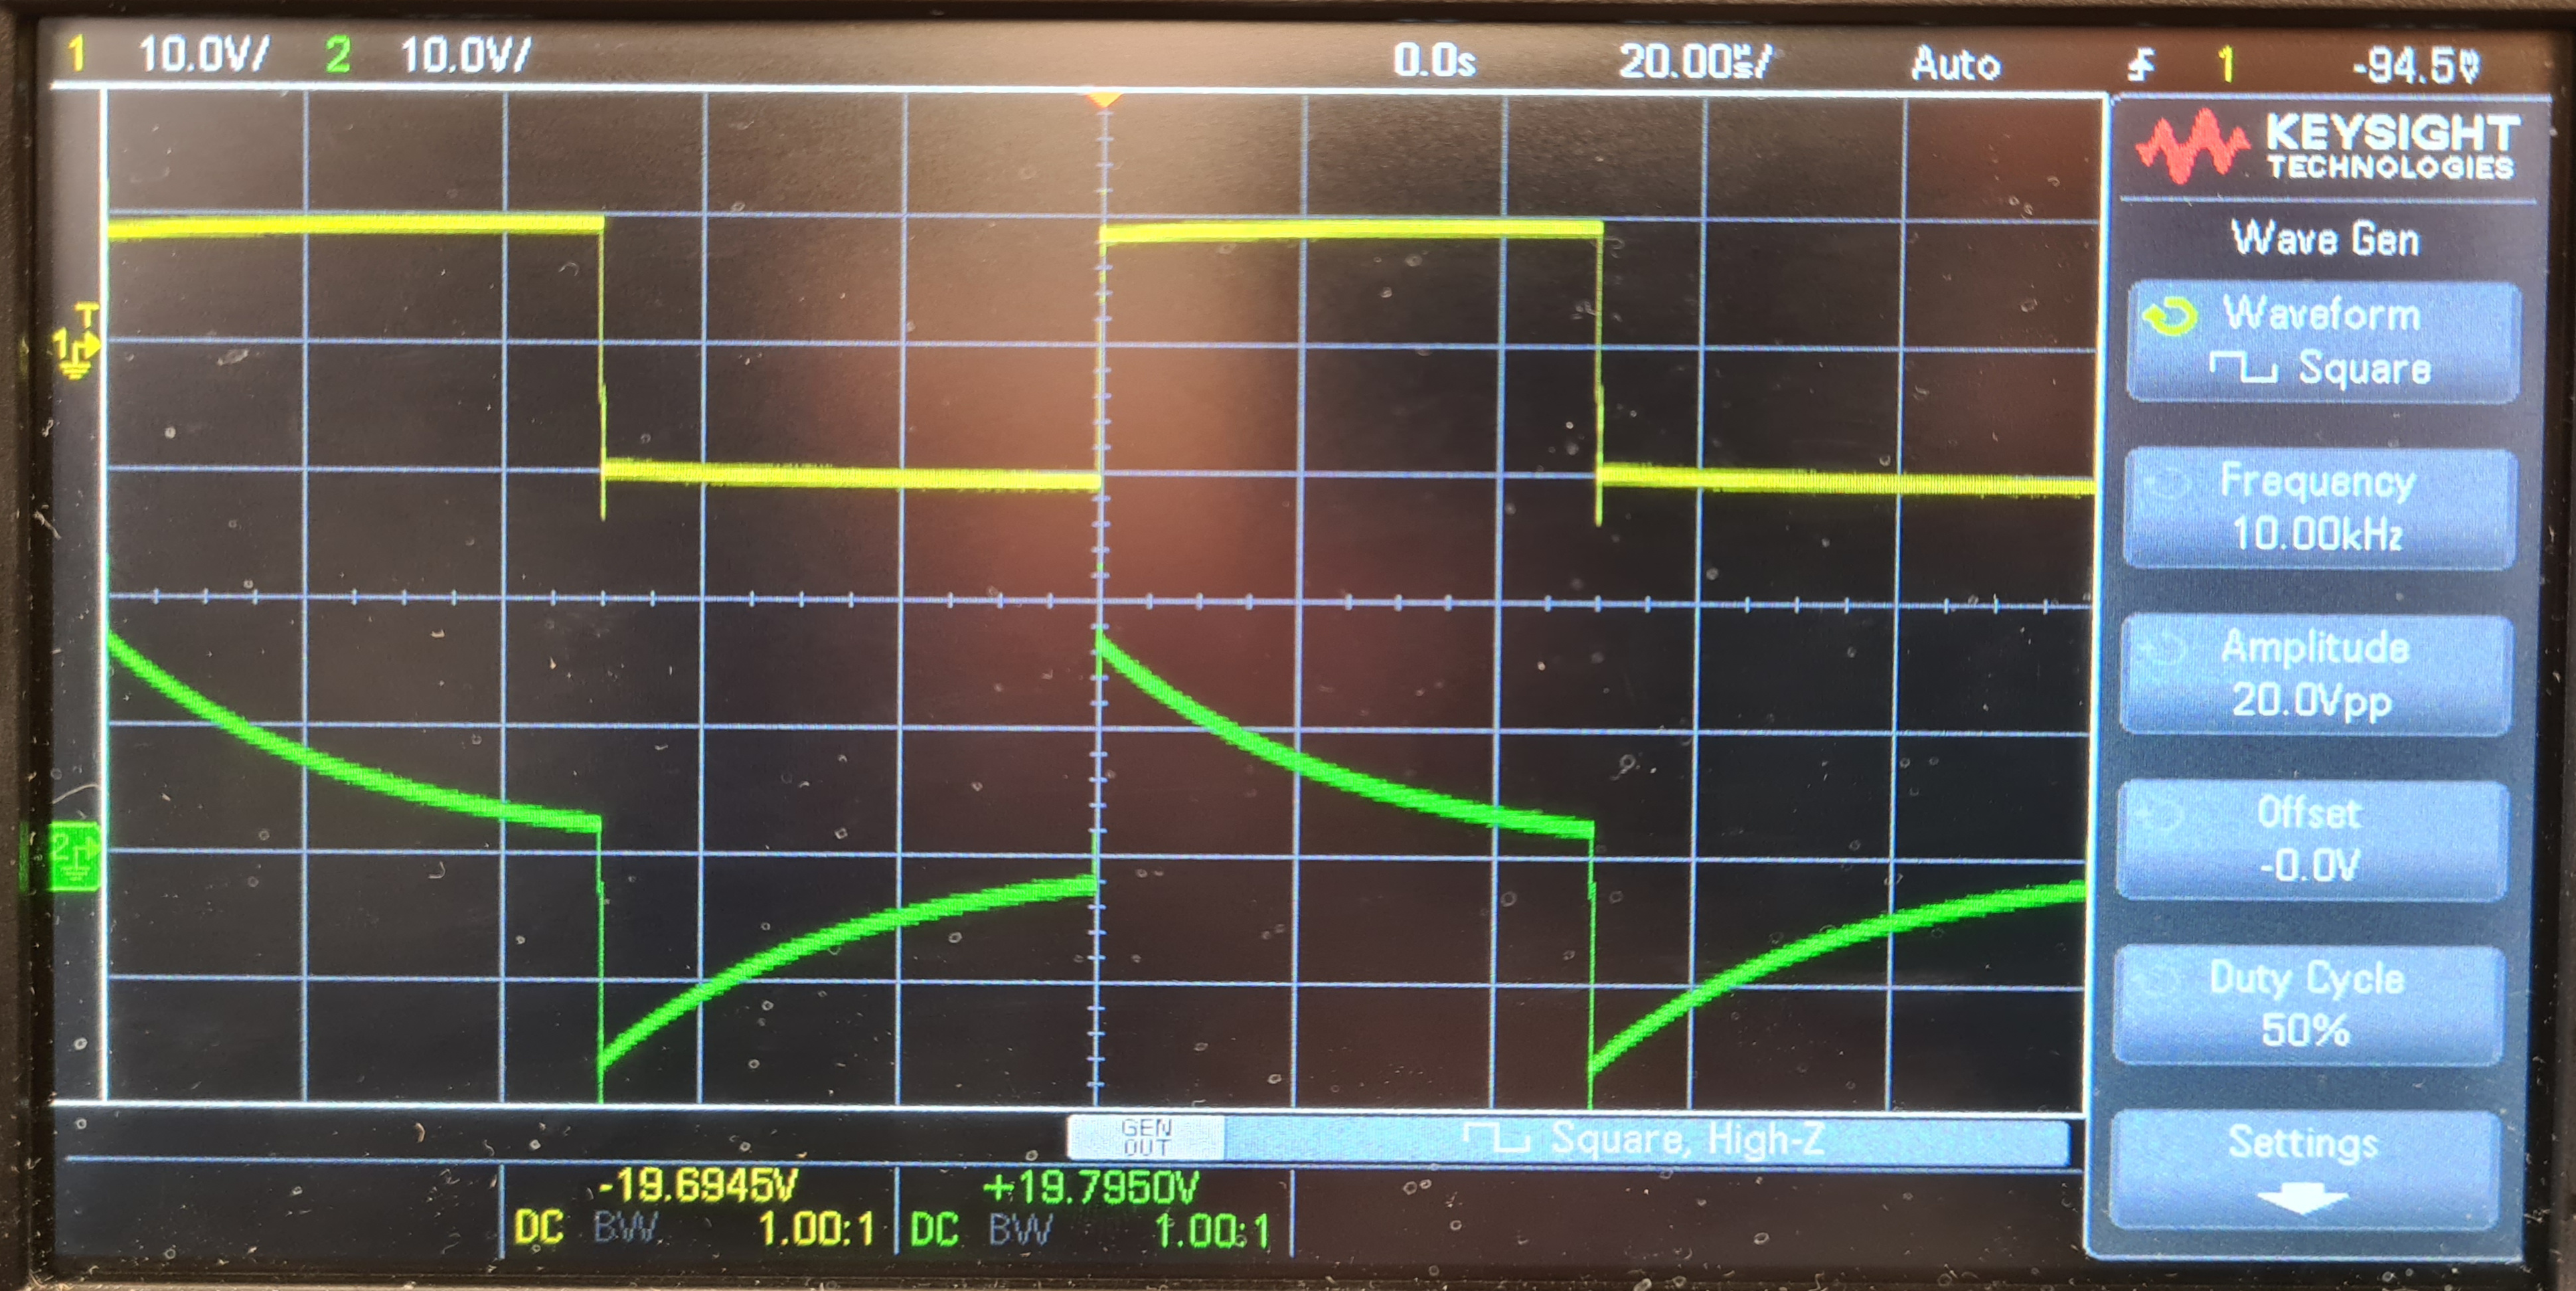
\includegraphics[width=.9\linewidth]{../data/20211116_104029-mod.jpg}
    \caption{RC Circuit with Square Wave}
  \end{subfigure}%
  \begin{subfigure}{.5\textwidth}
    \centering
    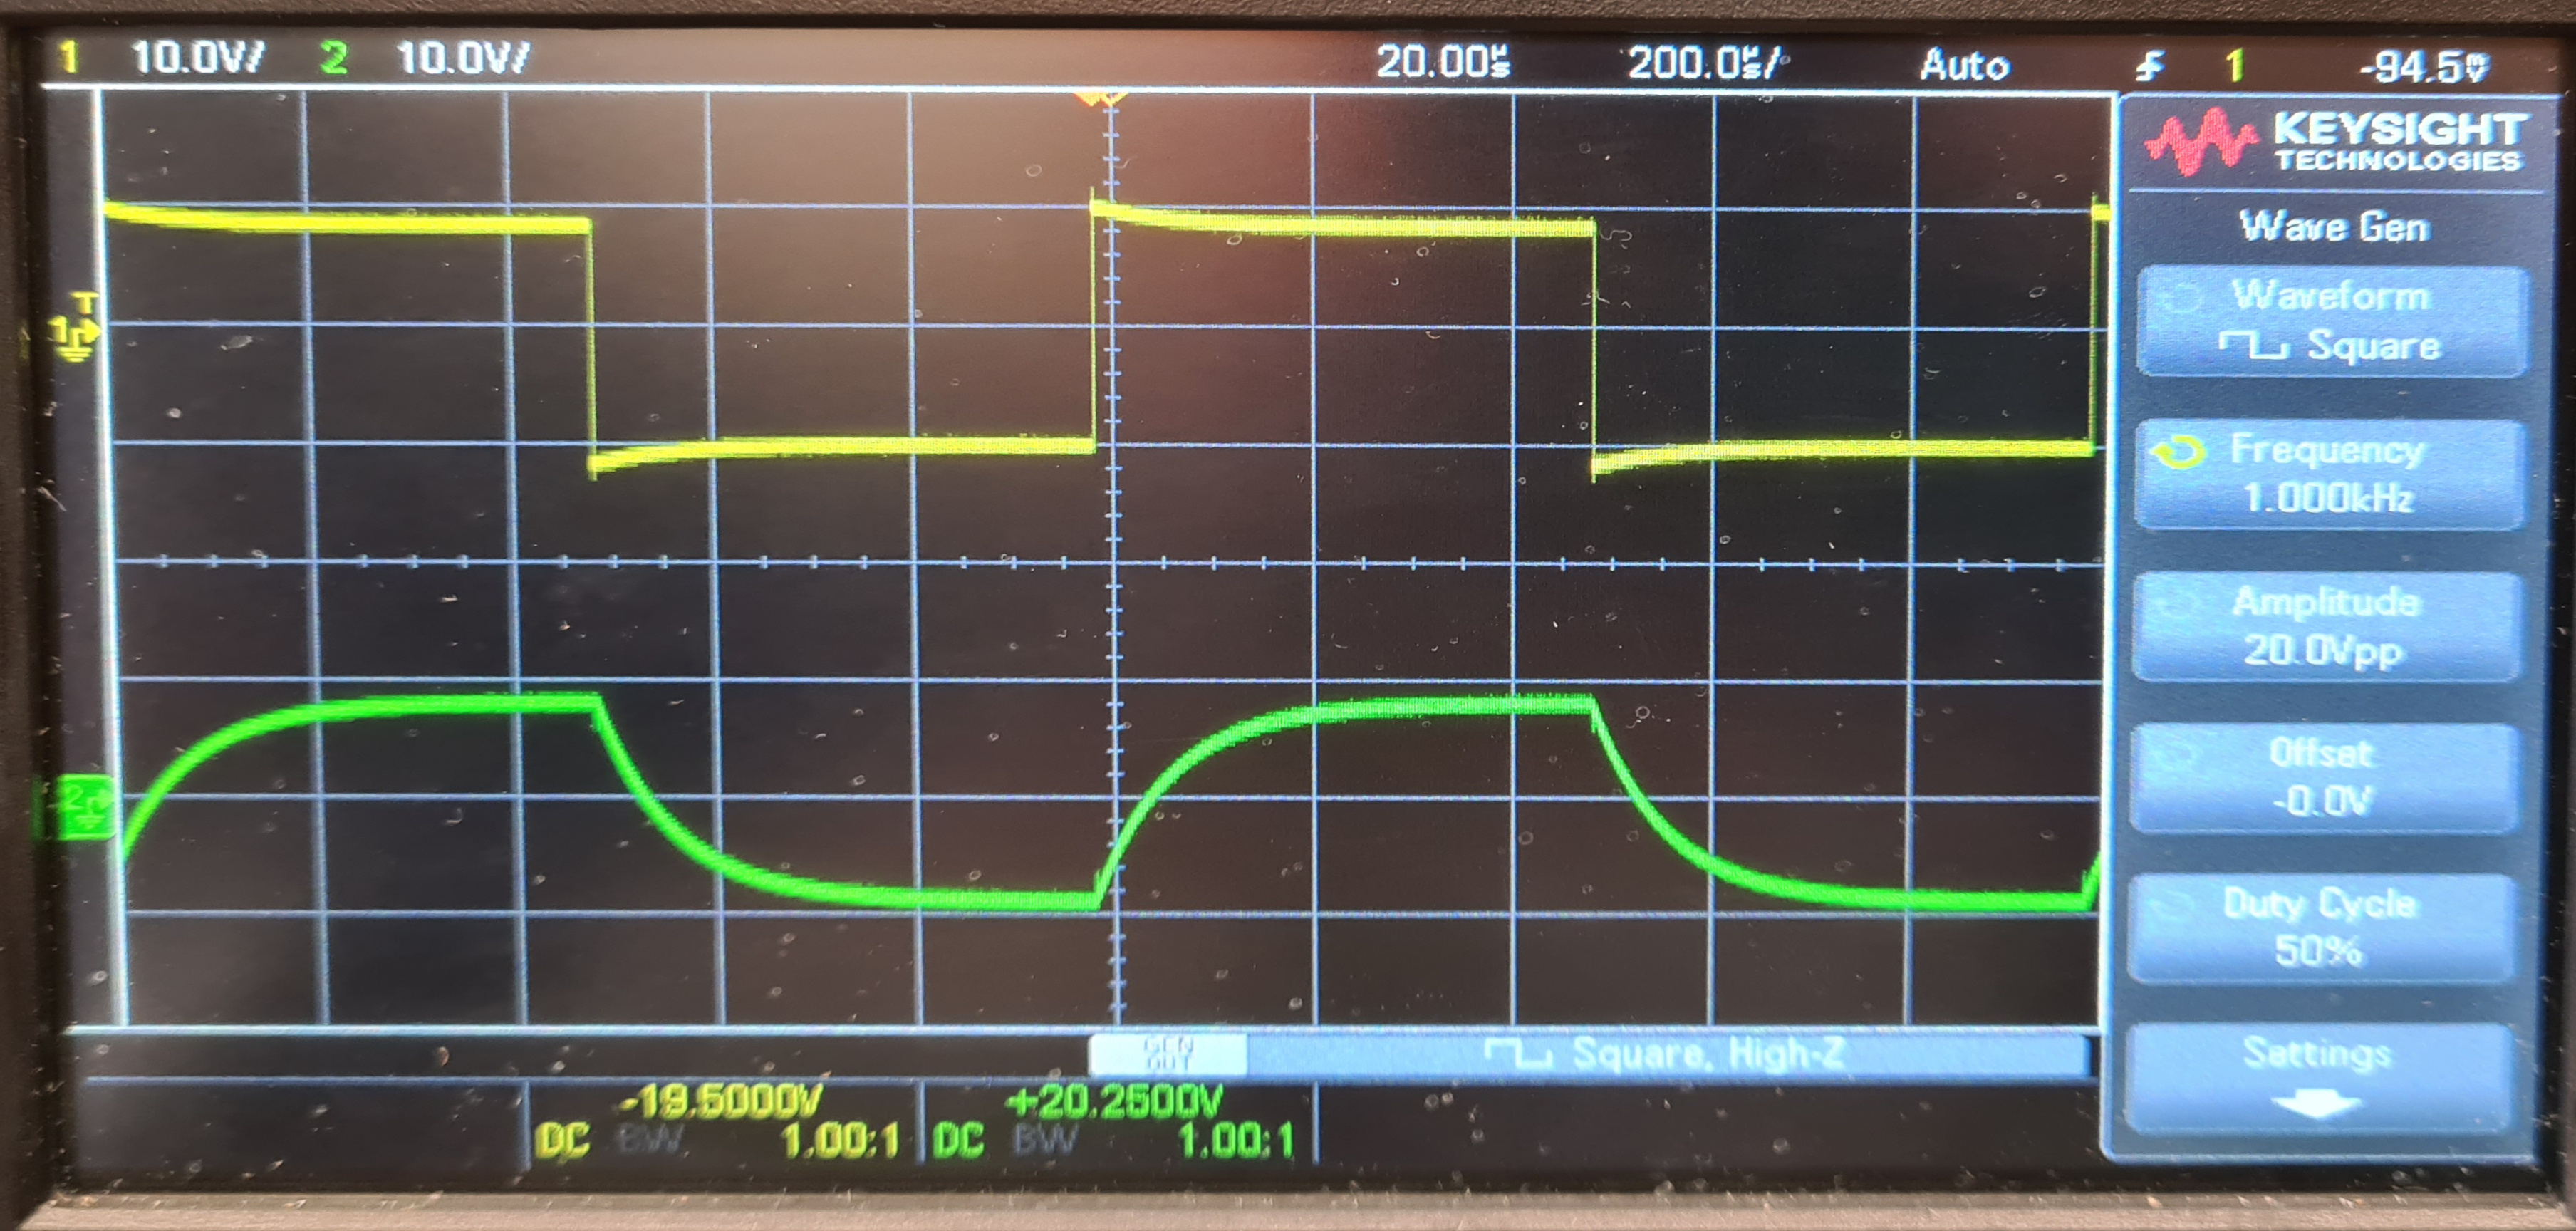
\includegraphics[width=.9\linewidth]{../data/20211116_104711-mod.jpg}
    \caption{LR Circuit with Square Wave}
  \end{subfigure}
\end{figure}

\pagebreak

\subsection{Experimental Data}

\subsubsection{RC Sine Wave}
\verbatiminput{../data/rc_sine.csv}

\subsubsection{LR Sine Wave}
\verbatiminput{../data/lr_sine.csv}

\subsubsection{LCR Sine Wave}
\verbatiminput{../data/lcr_sine.csv}

\pagebreak

\subsection{Python Code}

\subsection{Simulated Curves}

\verbatiminput{../Simulated Curves/Simulated curves.py}
\noindent\rule{\textwidth}{1pt}

\pagebreak

\subsection{Impedance and Phase Plots}

The Python code for this exercise is divided into two files. The statslab.py file contains utility methods
which we will be frequently using in this course. The lab\_7.py file contains the code which analyzes
the data.

\subsubsection{statslab.py}
\noindent\rule{\textwidth}{1pt}
\verbatiminput{../code/statslab.py}
\noindent\rule{\textwidth}{1pt}

\pagebreak

\subsubsection{lab\_7.py}
\noindent\rule{\textwidth}{1pt}
\verbatiminput{../code/lab_7.py}
\noindent\rule{\textwidth}{1pt}


\pagebreak

\begin{thebibliography}{99}

\bibitem{lab-manual-ex7} Currents in LCR - currents-l-c-r.pdf (\url{https://q.utoronto.ca/courses/235154/files/15436318/download?wrap=1}).

\end{thebibliography}

\end{document}
